\section{Effectiveness of the approach}\label{ms:sec:security}

In this section, we elaborate on the effectiveness of our approach for enforcing revocation. For the discussion, we recall that \msize\ is the size of individual mini-blocks, \mnumb\ is the number of mini-blocks in a block, \bnum\ is the number of blocks in a macro-block, and \Mnum\ is the number of macro-blocks. Also, we denote with \fnum\ \! the number of fragments, that is, $\fnum=\mnumb \cdot \bnum$.

We consider the threat coming from a user whose access to the resource has been revoked, and who downloads the resource from the server. With access policy enforced by encryption, not being authorized for an access should not prevent downloading the resource but rather it should prevent reconstruction of its plaintext representation. We then evaluate the protection against the user's attempts to reconstruct the plaintext resource. In doing so, we consider the worst case scenario, with respect to key management, where the user has maintained memory of the last key (or the corresponding seed) used for the resource up to the point in which she was authorized for the access. In other words, we assume the user to be able to decrypt the fragments that have been overwritten before she has been revoked access, and hence to know the original version encrypted with \key{0} of the fragments that have not been overwritten since she has been revoked access. Since seeds are compact, such a threat is indeed realistic. To reconstruct the resource when missing a fragment, the user would have to perform a brute force attack attempting all possible combinations of values of the missing bits, that is, $2^{\tiny\msize}$ attempts for each of the \Mnum\ macro-blocks. If more fragments, let's say \fmiss, are missing, the user would have to perform $2^{\tiny{\msize}\cdot \fmiss}$ attempts for each of the \Mnum\ macro-blocks. 

The inability of the user to reconstruct a resource if some fragments have been overwritten is because, without such fragments, the user cannot retrieve the corresponding original version (the one encrypted with \key{0}) needed to correctly reconstruct the resource plaintext. A potential threat can then come if the user maintains a local storage with the original version of part of the resource. We distinguish two cases, depending on whether the user stores complete fragments or portions of them across the whole resource.

\begin{figure}[!t]
\begin{small}
\hrule          %
\begin{tabbing}
\hfill\\
{\bf Revoke}\\[1em]
\num{~~\!1:~}\= randomly select a fragment $\fragment{i}{}$ of \resource  \comm{fragment to be rewritten}\\[0.3em]
\num{~~\!2:~} \1 download $\fragment{\var{i}}{\var{c}}$ from the server \comm{version of the fragment stored}\\[0.3em]
\num{~~\!3:~} \1 {\bf if} \= $c> 0$ \mythen \comm{\fragment{\var{i}}{0} has been overwritten in a revocation} \\[0.3em]
\num{~~\!4:~} \2 derive key \key{c} \comm{derive \key{c} using key regression}\\[0.3em]
\num{~~\!5:~}  \2 $\fragment{\var{i}}{0}$ := \dec{\key{c}}{\fragment{\var{i}}{\var{c}}} \comm{retrieve the original version of the fragment}\\[0.3em]
\num{~~\!6:~} \1 determine the last key \key{l-1} used \comm{it is stored in  \resource's descriptor}  \\[0.3em]
\num{~~\!7:~} \1 generate new key \key{l} \\[0.3em]
\num{~~\!8:~} \1 \fragment{\var{i}}{\var{l}} := \enc{\key{l}}{\fragment{\var{i}}{0}}\\[0.3em]
\num{~~\!9:~} \1 upload \fragment{\var{i}}{\var{l}} overwriting $\fragment{\var{i}}{\var{c}}$ \comm{overwrite previous version}\\[0.3em]
\num{10:~} \1 encrypt \seed{l} with the key of {\em acl\/}(\resource) \comm{limits it to authorized users}\\[0.3em]
\num{11:~} \1 update  \resource's descriptor \comm{including the new \seed{l}}
\end{tabbing}
\hrule
\vspace{.5em}
\end{small}
\caption{\label{ms:fig:revoke}Revoke on resource \resource}
\end{figure}

\subsection{Local storage of fragments}
Suppose a user locally stores (when authorized) some fragments of the resource. Even if such fragments are later overwritten for revoking access to the user, and then their most recent version stored at the server is unintelligible to her, she has them available for reconstructing the resource. However, the fragment to be overwritten in a policy revocation is chosen randomly by the owner. Therefore, the user can still reconstruct the resource after one fragment has been overwritten if the fragment that the owner has overwritten is the same fragment that the user has also stored locally, which has probability ${1}/{\fnum}$ to occur. Generalizing the reasoning to the consideration of the user locally storing more than one fragment and the policy naturally changing even after the specific user revocation, we determine the probability $P_A$ of the user's ability to access the resource assuming local storage of \floc\ fragments to be $P_A=(\floc/\fnum)^{\fmiss}$. The probability clearly increases with the number of fragments stored locally, but quickly reaches extremely low values after a few updates of the policy, approximating zero even for high percentage of fragments locally stored. The low probability (and the high storage effort requested to the user) essentially makes such attack not suitable: if the user has to pay a storage cost that approaches the maintenance of the whole resource, then the user would have stored the plaintext resource when authorized in the first place. We note also that a possible extension of our approach could consider overwriting, instead of pre-defined fragments, a randomly chosen set of mini-blocks (ensuring coverage of all macro-blocks), to enforce a revocation. In this case, the probability of the user storing \mloc\ mini-blocks per macro-block (also randomly chosen) to be able to access the resource immediately after her revocation would be $(\mloc/(\mnumb\cdot\bnum))^{\Mnum}$, which would become $(\mloc/(\mnumb\cdot\bnum))^{\Mnum\cdot \mmiss}$, (i.e., negligible), if she misses \mmiss\ mini-blocks per macro-block. We note however that overwriting randomly picked mini-blocks across the resource would considerably increase the complexity in the management of fragments, and it would make it harder to provide an efficient physical structure for fragments (Section~\ref{ms:sec:expe}). Given the observations above about the high storage cost that would be required to the user and the low probability of her success as policy changes, we argue that the regular structure for the fragments is preferable.

\begin{figure}[!t]
\begin{small}
\hrule          %
\begin{tabbing}
\hfill\\
{\bf Access}\\[1em]
\num{~~\!1:~}\= download \resource's descriptor and all its fragments \\[0.3em]
\num{~~\!2:~}\1 retrieve seed \seed{l} used for the last encryption \\[0.3em]
\num{~~\!3:~}\1 compute keys $\key{0},\ldots,\key{l}$\\[0.3em]
\num{~~\!4:~}\1 \myfor\  each downloaded fragment \fragment{\var{i}}{\var{x}} \com{do} \\[0.3em]
\num{~~\!5:~}\2     {\bf if} $x>0$ {\bf then} \\[0.3em]
\num{~~\!6:~}\2     \fragment{\var{i}}{0} := \dec{\key{x}}{\fragment{i}{\var{x}}} \comm{retrieve the original version of fragments}\\[0.3em]
\num{~~\!7:~}\1 \myfor\ $j=0,\ldots,\Mnum-1$ \com{do} \comm{reconstruct and decrypt macro-blocks}\\[0.3em]
\num{~~\!8:~}\2     \macroblock{\var{j}} := concatenation of mini-blocks \fragment{\var{i}}{0}[\var{j}], $i=0,\ldots, (\mnumb \cdot \bnum)-1$\\[0.3em]
\num{~~\!9:~}\2     decrypt \macroblock{\var{j}}
\end{tabbing}
\hrule
\vspace{.5em}
\end{small}
\caption{\label{ms:fig:access}Access to resource \resource}
\end{figure}

\subsection{Keeping portions of all mini-blocks}
Instead of locally storing some selected fragments, a user can opt for using storage to maintain portions of all the mini-blocks in each fragment. In this case, whatever the fragment overwritten in the revocation, the user will have to perform some effort to realize a brute-force attack to retrieve the missing bits (she does not have the complete fragment), but such an effort will be lower, given the availability of the locally stored bits. For instance, assuming the user to keep 50\% (i.e., half of the bits) of each mini-block, the effort for reconstructing the resource given a missing fragment would now be $2^{\tiny{(\msize/2)}}$ attempts for each of the $M$ macro-blocks (in contrast to the $2^{\tiny\msize}$ required if all the bits in the fragment were unknown). However, again, if more fragments are missing, the required effort would quickly escalate, being equal to $2^{\tiny{(\msize/2)}\cdot \fmiss}$ when \fmiss\ fragments are missing. For each attempt, the verification that a guess is correct would require to apply all the decryption rounds until the plaintext is reconstructed, with a great cost. We note that the user can cut down on such cost if she locally maintains, in addition to the portions of the original mini-blocks, also some bits of the partial results of the computation (which would allow her to test correctness of a guess without performing all the encryption rounds). Availability of such partial results can help testing the guesses for a mini-block if the other mini-blocks in the same block are available (i.e., when the user misses only one fragment per block). However, from the birthday paradox, we note that the probability of two revocations hitting the same block (but a different fragment) quickly increases with the number of revocations. Then, after a few updates the advantage of the user keeping partial results of the computation will become ineffective. In addition to this, we note that, in this case as well, the storage and computational efforts required to the user do not seem to make this attack much preferable for her with respect to the choice of locally storing the whole plaintext resource itself in the first place.

\subsection{A note on collusion}
Collusion can happen when two users join effort to gain access to a resource that neither of them can access (we do not consider collusions with the server, which is assumed trustworthy to enforce the re-writing requested by the owner). In fact, if one of the users is authorized for the resource, she has no incentive and therefore there is no collusion. Also, the case of users working together to grant each other access to resources on which they individually have authorization cannot be considered collusion, since merging their knowledge they collectively do not go beyond their privileges. Collusion is then represented by users who join effort in maintaining portions of the resource (e.g., fragments or parts of mini-blocks as discussed above). For instance, each of the users could keep half of the fragments and they can merge their knowledge to patch for missing fragments. Such a situation does not add any complication with respect to the previous discussion, as it simply reduces to consider the group of colluding users as an individual attacker. We then note again that the collective effort, in terms of storage and/or computation, required to gain access would easily approximate the effort of locally storing the original plaintext resource itself. In other words, the attack strategy does not offer an advantages to users attempting to access the resources for which they are not authorized.

\new{

\subsection{A note on erasure coding}\label{ms:sect:erasure}
Cloud storage providers have to offer reliability to their users. To reach this goal, the easiest approach is to replicate data \cite{Calder:2011:WAS:2043556.2043571}. Yet, this requires a not negligible storage overhead.
Another less expensive approach is to leverage erasure coding \cite{huang2012erasure}. With this solution, data are divided into fragments and stored replicated together with a certain number of parity fragments. Erasure codes offer the same fault tolerance property with lower replication.

Even if the cloud provider does not use erasure coding, an adversary could build a client-side erasure coding that permits to mitigate the loss of a fragment (i.e., the loss of the ability to decrypt a fragment that has been re-encrypted due to a policy update that revokes the user). This means that, given a resource divided into $k$ fragments, the adversary can locally store $t$ (with $t < k$) parity fragments to be able to recover the plaintext of the resource as long as no more than $t$ different fragments have been re-encrypted.
%For instance, if we consider a resource divided into $k = 16$ fragments, an adversary could download the entire resource, build an erasure coding with $t = 2$ parity fragments, in order to be able to recover the resource even if she is revoked, as long as less than 2 different fragments are re-encrypted with a new key.
Yet, the resource owner has control over the number $r$ of fragments that she is willing to re-encrypt, and this nullifies the efforts made by the adversaries that stored a number of parity fragments smaller than $r$.

When the policy changes, the owner can promptly re-encrypt a single fragment to revoke access for common adversaries without local erasure codes. After this, the owner can still re-encrypt other random fragments, later in time. An adversary that has used erasure coding would need to know that the re-encryption process is happening and to quickly download the resource that is being re-encrypted to make use of its erasure code. This is a very error-prone and lucky-based process for the adversary to complete. Moreover, it is important to note that the adversary had access to the whole resource previously, so if it was important and compact, she would have stored the resource in plaintext.

\subsection{Comparison with other AONTs}

We can now better illustrate the differences between \name and other All-or-Nothing Transforms.

In general, other AONTs make use of two keys, the first is the encryption key, and the second is the AONT key. For example, the AONT proposed by Rivest in \cite{r97} applies a transformation on the plaintext before encryption. This transformation is similar to encrypting in counter mode, except that the key is randomly chosen rather than fixed, and the last ciphertext block is the exclusive-or of the key and a hash of all the other ciphertext blocks. This effectively ensures that if a ciphertext block is missing, the AONT key is lost and the transformation is not invertible, thus realizing an AONT.

This schema works in the network transmission setting but can be easily circumvented in the access revocation scenario. An adversary could store the AONT key and thus be able to invert the transformation even if a fragment has been updated. The missing fragment implies missing parts in the plaintext, however, the majority of it would still be accessible.
This scenario gets even worse in case the adversary has kept a local erasure code (as in Section~\ref{ms:sect:erasure}). Let's assume that the adversary has kept an erasure code as big as $a\%$ of the resource size, and that the owner is re-encrypting $r\%$ due to a policy update.

In case $r < a$ (i.e., the policy update re-encrypts a portion of the resource whose size is smaller than the adversarial erasure code), then the revoked user can still access the file in its integrity in both Rivest's AONT and \name.

\noindent When $r \geq a$, instead, we have the following two scenarios.

\begin{description}
	\item [Rivest's AONT] The user can apply its erasure code, then use the AONT key to invert the function and re-gain access to a portion of the size as big as $1 - (r - a)$.
	\item [\name] Even after applying the erasure code, there is no key that can be used to invert the function, and the entire contents of the file are lost.
\end{description}

\begin{figure}[t]
	\centering
	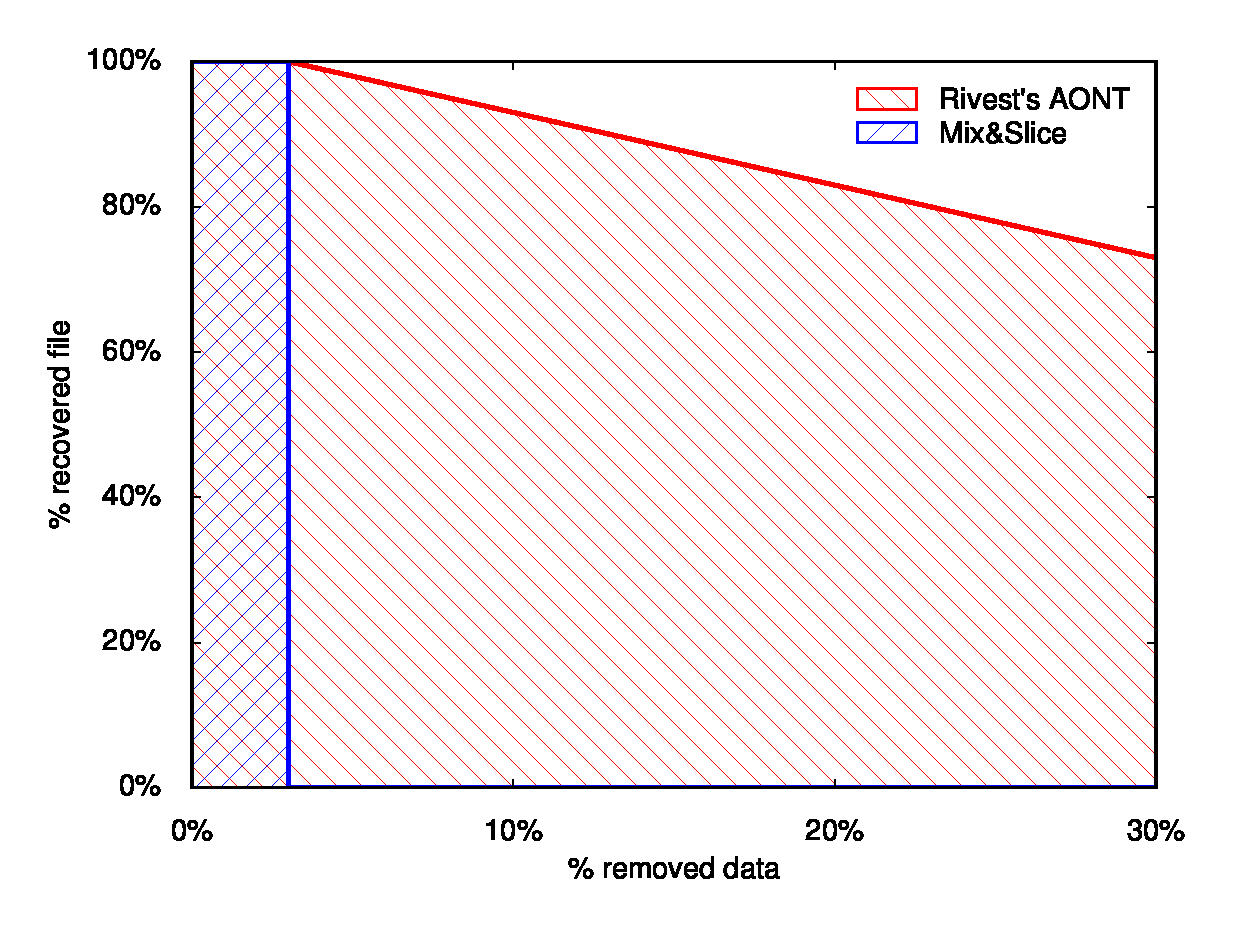
\includegraphics[width=0.75\columnwidth]{figures/experiments/out}
	\caption{Comparison of percentage of recovered file between Rivest's AONT and \name when the revoked user has kept an erasure code whose size is 3\% of the resource size}
	\label{ms:aont-comparison}
\end{figure}

\noindent This property is depicted in Figure~\ref{ms:aont-comparison}.

} % end \new
